\documentclass[12pt]{exam}
\usepackage[utf8]{inputenc}
\usepackage{amsmath,amstext,amsthm,amssymb,amsxtra, graphicx}
\usepackage[top=1.5in, bottom=1.5in, left=1.25in, right=1.25in]	{geometry}
%\usepackage[normalem]{ulem}
\usepackage{cancel}
\usepackage{txfonts} % pxfonts txfonts 
\usepackage[T1]{fontenc}
\usepackage{lmodern}
\renewcommand*\familydefault{\sfdefault}
 \usepackage{euler}   % better than the option below
\usepackage{pdfsync}
\usepackage{multicol}
\newcommand{\ci}[1]{_{ {}_{\scriptstyle #1}}}
\graphicspath{ {images/} }
\usepackage{pdfpages}


\newcommand{\norm}[1]{\ensuremath{\left\|#1\right\|}}
\newcommand{\abs}[1]{\ensuremath{\left\vert#1\right\vert}}
\newcommand{\ip}[2]{\ensuremath{\left\langle#1,#2\right\rangle}}
\newcommand{\p}{\ensuremath{\partial}}
\newcommand{\pr}{\mathcal{P}}

\newcommand{\pbar}{\ensuremath{\bar{\partial}}}
\newcommand{\db}{\overline\partial}
\newcommand{\D}{\mathbb{D}}
\newcommand{\B}{\mathbb{B}}
\newcommand{\Sp}{\mathbb{S}}
\newcommand{\T}{\mathbb{T}}
\newcommand{\R}{\mathbb{R}}
\newcommand{\Z}{\mathbb{Z}}
\newcommand{\C}{\mathbb{C}}
\newcommand{\N}{\mathbb{N}}
\newcommand{\Q}{\mathbb{Q}}
\newcommand{\mQ}{\mathcal{Q}}
\newcommand{\mS}{\mathcal{S}}
\newcommand{\scrH}{\mathcal{H}}
\newcommand{\scrL}{\mathcal{L}}
\newcommand{\td}{\widetilde\Delta}
\newcommand{\pw}{\text{PW}}
\newcommand{\esup}{\text{ess.sup}}
\newcommand{\Tn}{\mathcal{T}_n}
\newcommand{\Bn}{\mathbb{B}_n}
\newcommand{\rt}{\mathcal{O}}
\newcommand{\avg}[1]{\langle #1 \rangle}
\newcommand{\one}{\mathbbm{1}}
\newcommand{\eps}{\varepsilon}
\newcommand{\grad}{\nabla}

\newcommand{\La}{\langle }
\newcommand{\Ra}{\rangle }
\newcommand{\rk}{\operatorname{rk}}
\newcommand{\card}{\operatorname{card}}
\newcommand{\ran}{\operatorname{Ran}}
\newcommand{\osc}{\operatorname{OSC}}
\newcommand{\im}{\operatorname{Im}}
\newcommand{\re}{\operatorname{Re}}
\newcommand{\tr}{\operatorname{tr}}
\newcommand{\vf}{\varphi}
\newcommand{\f}[2]{\ensuremath{\frac{#1}{#2}}}

\newcommand{\kzp}{k_z^{(p,\alpha)}}
\newcommand{\klp}{k_{\lambda_i}^{(p,\alpha)}}
\newcommand{\TTp}{\mathcal{T}_p}
\newcommand{\m}[1]{\mathcal{#1}}
\newcommand{\md}{\mathcal{D}}
\newcommand{\qan}{\abs{Q}^{\alpha/n}}
\newcommand{\sbump}[2]{[[ #1,#2 ]]}
\newcommand{\mbump}[2]{\lceil #1,#2 \rceil}
\newcommand{\cbump}[2]{\lfloor #1,#2 \rfloor}

\newcommand{\hn}{{1}}
\newcommand{\dd}{{09-27}}
\newcommand{\class}{Aero 455}
\newcommand{\term}{Fall 2024}
\newcommand{\examnum}{Homework \hn: Due \dd}
\newcommand{\examdate}{}
\newcommand{\timelimit}{75 Minutes}
\newcommand{\vc}[3]{\langle #1,#2,#3\rangle}
\newcommand*{\vv}[1]{\vec{\mkern0mu#1}}
\newcommand{\bv}[1]{\boldsymbol{#1}}
\newcommand{\hide}[1]{}
\newcommand{\uvec}[1]{\boldsymbol{\hat{\textbf{#1}}}}
\newcommand{\vex}[1]{\boldsymbol{{\textbf{#1}}}}
\newcommand{\px}{\frac{\partial}{\partial x}}
\newcommand{\py}{\frac{\partial}{\partial y}}
\newcommand{\pt}{\frac{\partial}{\partial t}}
\newcommand{\pxx}{\frac{\partial^2}{\partial x^2}}
\newcommand{\pyy}{\frac{\partial^2}{\partial y^2}}
\newcommand{\ptt}{\frac{\partial^2}{\partial t^2}}


\pagestyle{head}
\firstpageheader{}{}{}
\runningheader{\class}{ Page \thepage\ of \numpages}{\examnum}
\runningheadrule

\makeatletter
\renewcommand*\env@matrix[1][*\c@MaxMatrixCols c]{%
  \hskip -\arraycolsep
  \let\@ifnextchar\new@ifnextchar
  \array{#1}}
\makeatother

\printanswers
\begin{document}

\noindent
\begin{tabular*}{\textwidth}{l @{\extracolsep{\fill}} r @{\extracolsep{6pt}} l}
\textbf{\class} & \textbf{Name:} & \makebox[2in]{\bf{Benjamin Tollison}}\\
\end{tabular*}\\
\rule[2ex]{\textwidth}{2pt}
%
\begin{questions}
\begin{question}
Using Bernoulli’s equation instead of general energy equation, prove that the induced
velocity in the fully contracted wake of a rotor climbing vertically is twice the induced
velocity in the rotor plane. You could use the mass and momentum equations. 

\end{question}
\begin{solutionorbox}[\stretch{1}]
\begin{align*}
\begin{cases}
P_0 + \frac{1}{2}\rho v_0^2 = P_1 + \frac{1}{2}\rho v_1^2 \\
P_2 + \frac{1}{2}\rho v_2^2 = P_3 + \frac{1}{2}\rho v_3^2 \\ 
v_0 = 0 \\
v_1 = v_2 = v_i \\ 
v_3 = w
\end{cases}
\end{align*}
\begin{align*}
\begin{cases}
\rho v_i \sigma_i = \rho w \sigma_w \\
T = \int_{\sigma_3}{\rho v_3 \left(v_3 \cdot n\right)}d\sigma_3 - \int_{\sigma_0}{\rho \cancelto{0}{v_0} \left(\cancelto{0}{v_0}\cdot n\right)}d\sigma_0
\end{cases}
\end{align*}
Simplifying the thrust equation produces
\begin{equation}
T = \rho v_3^2 \sigma_3 = \dot{m}w = \rho w^2 \sigma_3
\end{equation}
Using the relation of \(P_0 = P_3\) and plugging back into Bernoulli’s produces

\[P_0 + \cancelto{0}{\frac{1}{2}\rho v_0^2} = P_1 + \frac{1}{2}\rho v_i^2 \]
\[P_0 = P_1 + \frac{1}{2}\rho v_i^2 \]
\[P_2 + \cancel{\frac{1}{2}\rho v_i^2} = P_1 + \cancel{\frac{1}{2}\rho v_i^2} + \frac{1}{2}\rho w^2 \]
\[P_2-P_0 = \frac{1}{2}\rho w^2\]
and the difference of pressure can be defined as the thrust across the blade membrane
\begin{equation}
\frac{T}{\sigma_2} = \frac{1}{2}\rho w^2
\end{equation}
Plugging equation 1 into 2 gives
\[\frac{\rho w^2 \sigma_3}{\sigma_2} = \frac{1}{2}\rho w^2\]
\[\frac{\cancel{\rho w^2} \sigma_3}{\sigma_2} = \frac{1}{2}\cancel{\rho w^2}\]
\begin{equation}
\frac{\sigma_3}{\sigma_2} = \frac{1}{2}
\end{equation}
Plugging equation 3 into the conservation of mass
\[\frac{\sigma_2}{\sigma_3} = \frac{w}{v_i}\]
\[2 = \frac{w}{v_i}\]
\[\therefore w = 2 v_i\]
\end{solutionorbox}

\newpage 
\begin{question}
Measurements have been made of rotor performance at a fixed rotor speed for a series of
blade pitch angles. The values of \(C_T\) that were measured were 6.0000E-06, 0.0010490,
0.0023760, 0.0040760 and 0.0055810, and the corresponding values of \(C_P\) were 0.000197,
0.000226, 0.000282, 0.000405 and 0.000555, respectively. Plot this data in the form of a
power polar (\(C_T\) vs. \(C_P\)). Explain (and show in a chart) how to extract induced power factor
(\(\kappa\)) and zero thrust power (profile power) for the rotor from these measured data. Then, to
the experimental power polar chart add the analytical power polar curve predicted by
modified momentum theory
\end{question}
\begin{solutionorbox}[\stretch{1}]


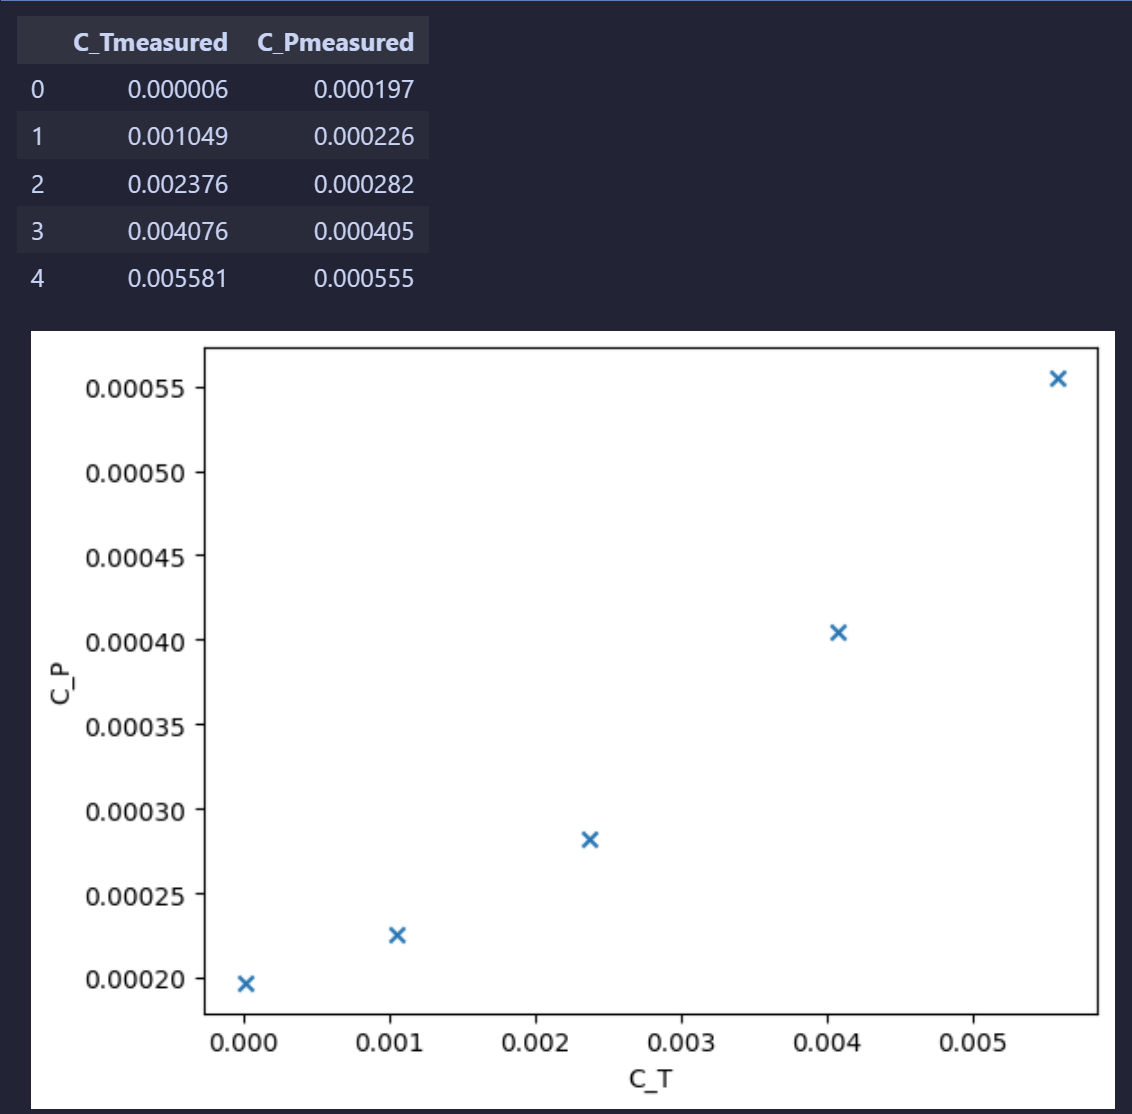
\includegraphics[width = \linewidth]{cp v ct measured.png}
Graphing momentum theory of \[C_P = \frac{C_T^{\frac{3}{2}}}{\sqrt{2}}\]
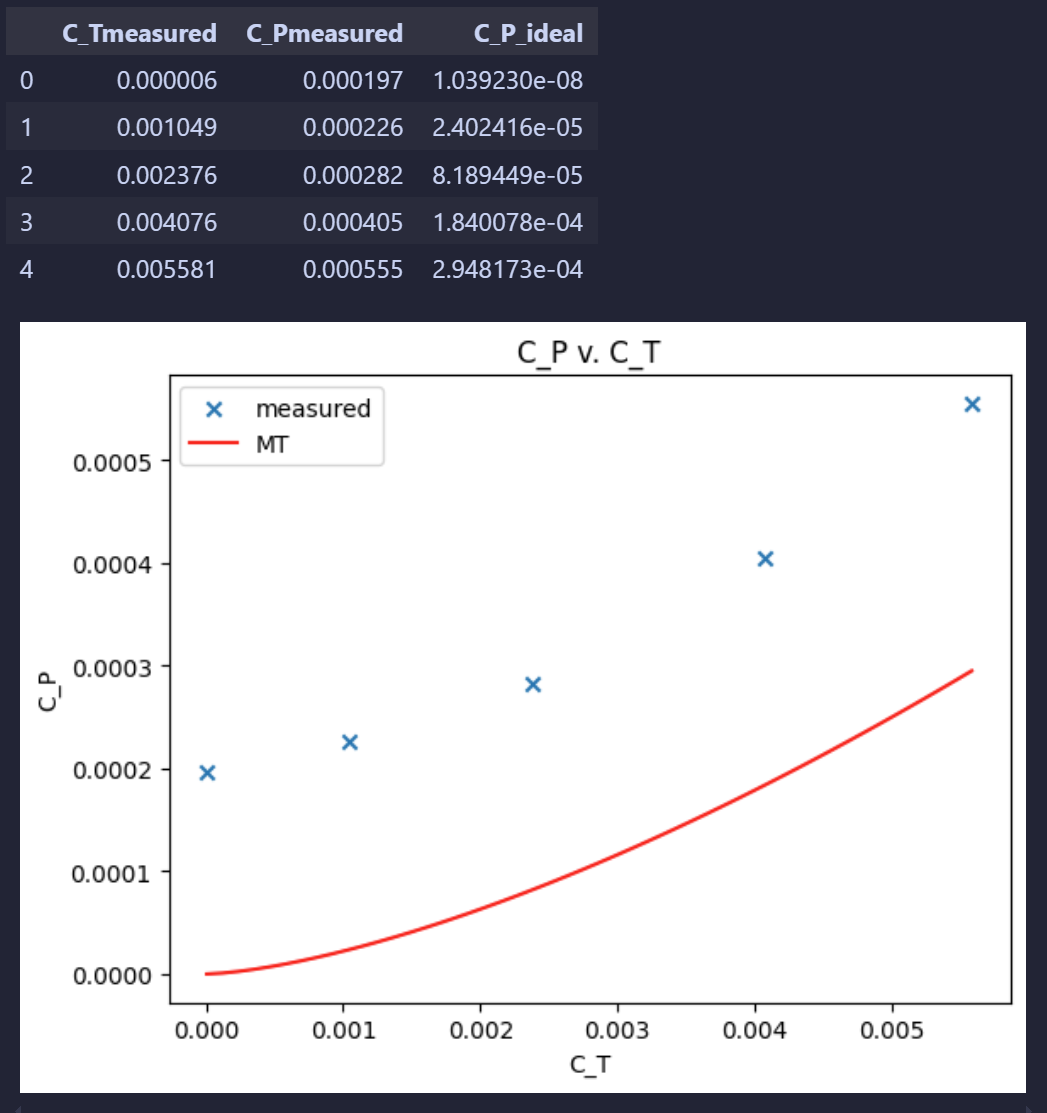
\includegraphics[width=\linewidth]{cp v ct mt.png}

\pagebreak
Normalizing the \(C_{P,ideal}\) with the measured values produces the following
graph and then finding the linear fit produces the following.

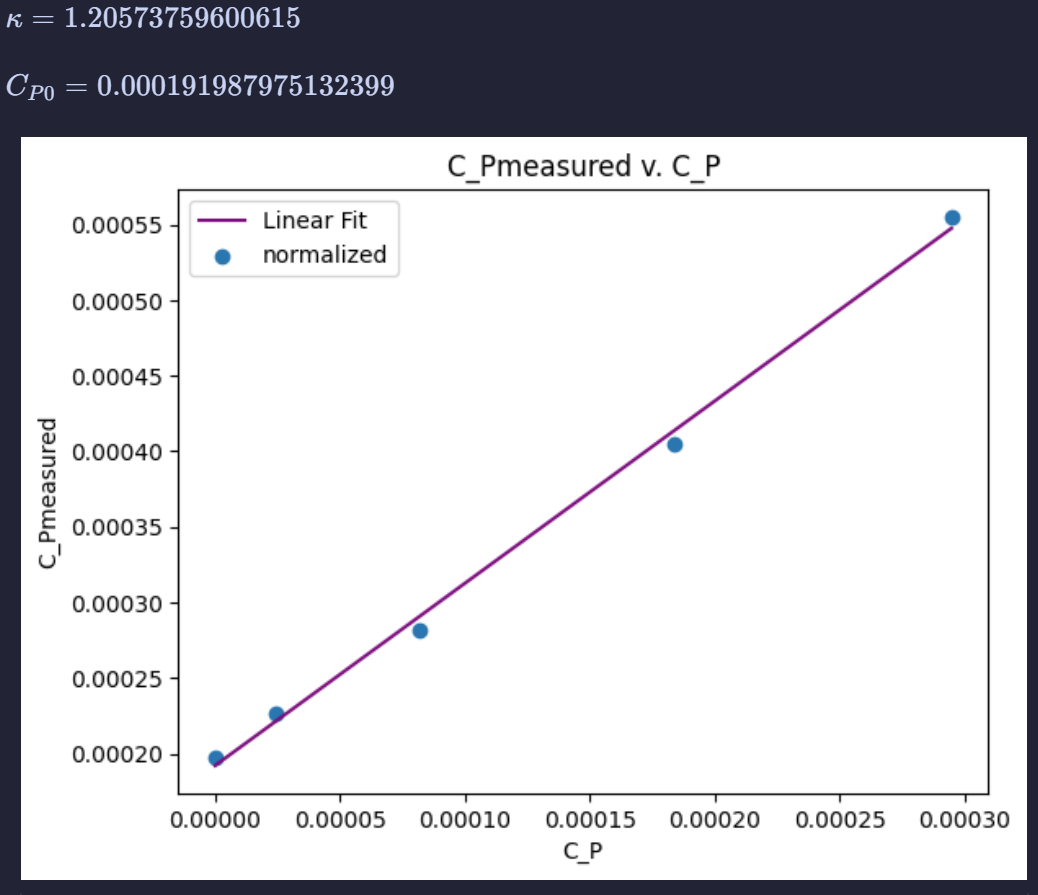
\includegraphics[width=\linewidth]{linear fit of cp.png}

\pagebreak
Creating the following modified momentum theory of 
\[C_P = \kappa\frac{C_T^{\frac{3}{2}}}{\sqrt{2}} + C_{P0}\]

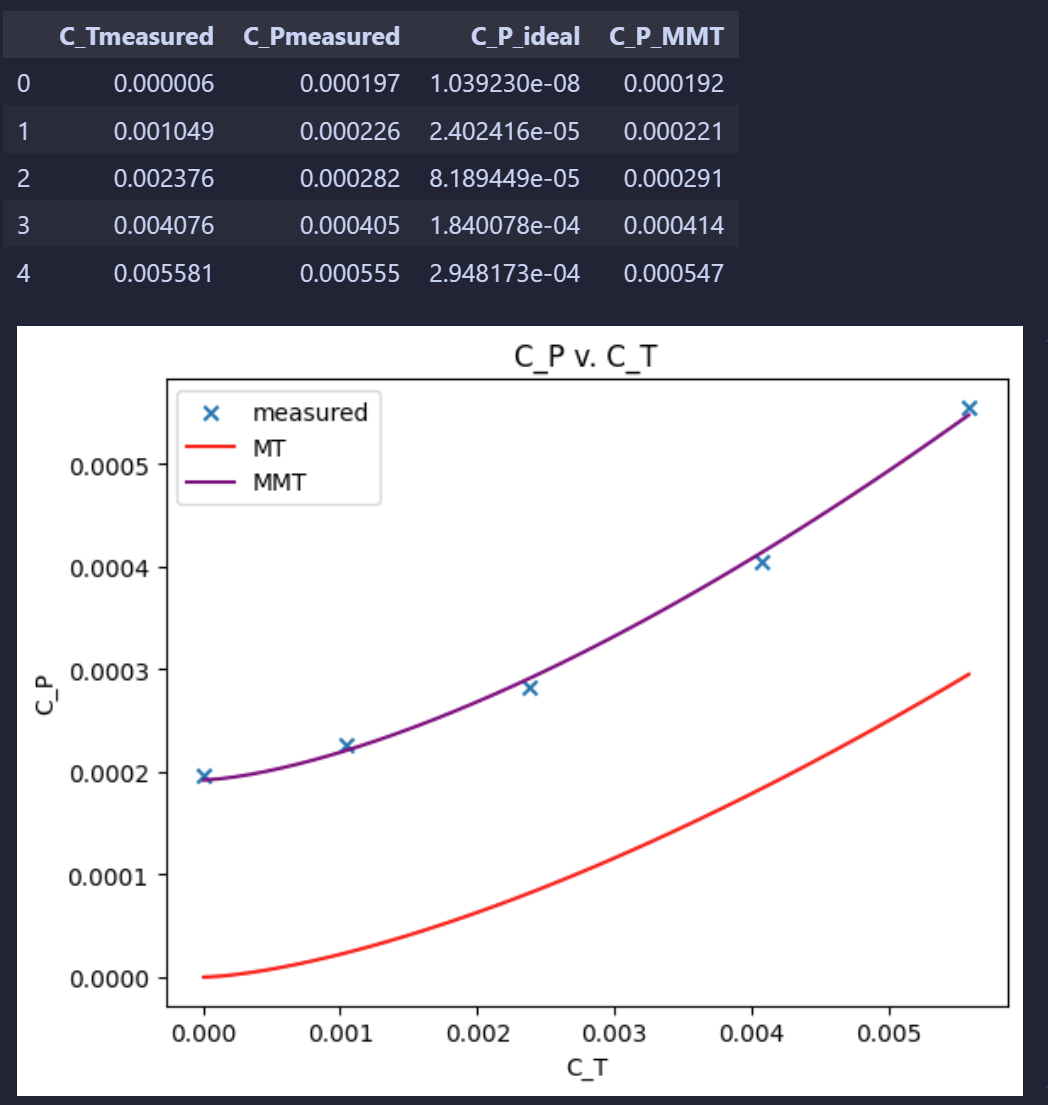
\includegraphics[width=\linewidth]{cp v ct mmt.png}

\end{solutionorbox}


\newpage 
\begin{question}
A helicopter with a gross weight of 3,000 lb (1,360.5 kg), a main rotor radius of 13.2 ft
(4.0 m), a rotor tip speed of 680 ft/s (207.3 m/s), and has 275 hp (205 kW) delivered to the
main rotor shaft. For hovering at sea level conditions, compute: (a) the rotor disk loading,
(b) the ideal power loading, (c) the thrust and torque coefficients, (d) the figure of merit
and actual power loading.
\end{question}
\begin{solutionorbox}[\stretch{1}]
a)
\[ T = mg \]
\[ \sigma = \pi R^2 \]
\[ \text{DL} = \frac{T}{\sigma} \]
\[\text{DL} = 265.520\]
b)
\[PL_{ideal} = \frac{T}{Tv_i} = \frac{1}{v_i} = \sqrt{\frac{2\rho}{DL}}\]
\[PL_{ideal} = 0.096058\]
c)
\[ C_T = \frac{T}{\rho\sigma(\Omega R)^2} \]
\[ C_{P,ideal} = \frac{P_h}{\rho\sigma(\Omega R)^3},C_{P,measured} = \frac{P}{\rho\sigma(\Omega R)^3} \]
\[C_Q = C_P\]
\[C_T = 0.0050439\]
\[C_{P,ideal} = 0.0002533\]
\[C_{P,actual} = 0.0003737\]
d)
\[ FM = \frac{P_h}{P_{actual}} = \frac{C_{P,ideal}}{C_{P,measured}} \]
\[ PL_{actual} = \frac{PL_{ideal}}{FM} \]
\[FM = 0.67777\]
\[PL_{actual} = 0.141727\]
\end{solutionorbox}


\newpage 
\begin{question}
For the helicopter described in the previous question, the tail rotor radius is 2.3 ft (0.701
m) and the tail rotor is located 15.3 ft (4.66 m) from the main rotor shaft. Calculate the
thrust and power required by the tail rotor when helicopter is hovering at sea level. Assume
that the figure of merit of the tail rotor is 0.7.
\end{question}
\begin{solutionorbox}[\stretch{1}]
\[ \tau = F \times r \]
\[ Q = T_{tail} \times r \]
\[ Q = C_{P,actual} \rho \sigma \left(\Omega R\right)^2 R \]
\[ \therefore T_{tail} = \frac{Q}{r} \]
\[ P = \frac{T_{tail}^\frac{3}{2}}{\sqrt{2\rho\sigma}} \]
\[T_{tail} = 848.8455 \text{[N]}\]
\[P_{tail} = 12716.4812 \text{[W]}\]
\end{solutionorbox}

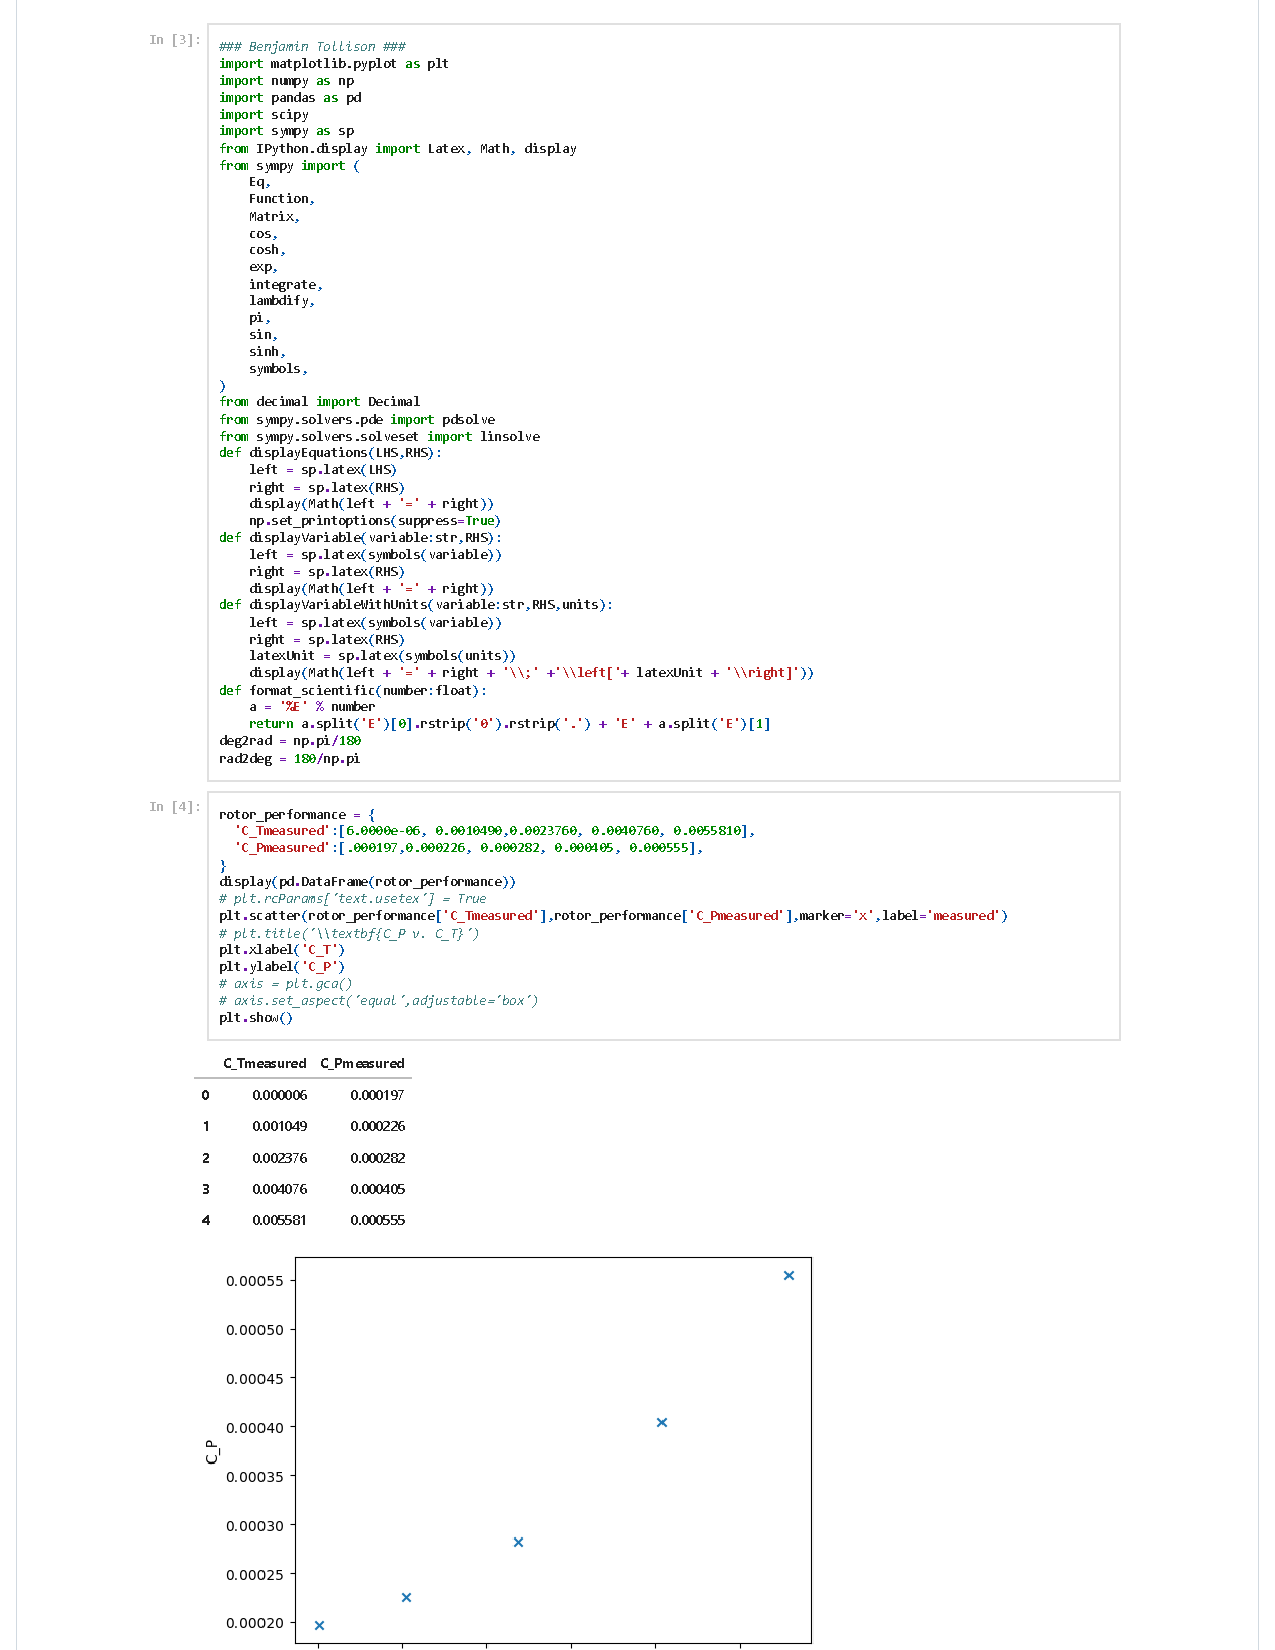
\includepdf[pages=-]{455 hw-1 calculations.pdf}

\end{questions}
\end{document}
